\newpage
\section{数理方程的建立和定解条件}
\subsection{典型偏微分方程的建立}
\subsubsection{弦的横振动}
\begin{figure}[htbp] %H为当前位置,!htb为忽略美学标准,htbp为浮动图形
    \centering %图片居中
    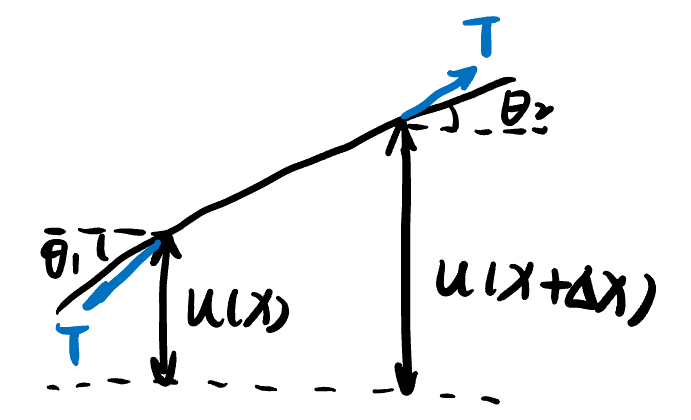
\includegraphics[width=0.3\textwidth]{figures/Rope.png} %插入图片,[]中设置图片大小,{}中是图片文件名
    \label{rope} %用于文内引用的标签
\end{figure}%结束环境
小振动:$\cos\theta\approx1$,忽略$\theta^2$量级;$\sin{\theta}\approx\tan{\theta}\approx\theta=
\frac{\partial{u}}{\partial{x}}$,忽略$\theta^3$量级

x方向合力:
$$F_x=T\cos{\theta_2}-T\cos{\theta_1}=0$$

u方向合力:
$$
    F_{\mbox{合}}=T\sin{\theta_2}-T\sin{\theta_1}
    \approx T\left(\frac{\partial{u}}{\partial{x}}|_{x+\Delta x}-\frac{\partial{u}}{\partial{x}}|_x\right)
    \approx T \frac{\partial^2{{u}}}{\partial{x}^2}\Delta x
$$

根据牛二定律:($ \dfrac{\partial^2{\bar{u}}}{\partial{t}^2}$:质心加速度)
$$F_{\mbox{合}}=\Delta m\frac{\partial^2{\bar{u}}}{\partial{t}^2}=\rho\Delta x\frac{\partial^2{\bar{u}}}{\partial{t}^2}$$
$$$$

结合两式,得到波动方程
$$T \frac{\partial^2{u}}{\partial{x}^2}=\rho\frac{\partial^2{u}}{\partial{t}^2}$$

作变量代换$a=\sqrt{\dfrac{T}{\rho}}$
$$\boxed{\frac{\partial^2{u}}{\partial{t}^2}=a^2\frac{\partial^2{u}}{\partial{x}^2}}$$

推广:二维均匀弹性膜横振动
$$\frac{\partial^2{u}}{\partial{t}^2}=a^2\left(\frac{\partial^2{u}}{\partial{x}^2}+\frac{\partial^2{u}}{\partial{y}^2}\right)$$
$$\left(\nabla^2-\frac{1}{a^2}\frac{\partial^2}{\partial{t}^2}\right)u(\vec{r},t)=0$$

\subsubsection{杆的纵振动}

\begin{figure}[H] %H为当前位置,!htb为忽略美学标准,htbp为浮动图形
    \centering %图片居中
    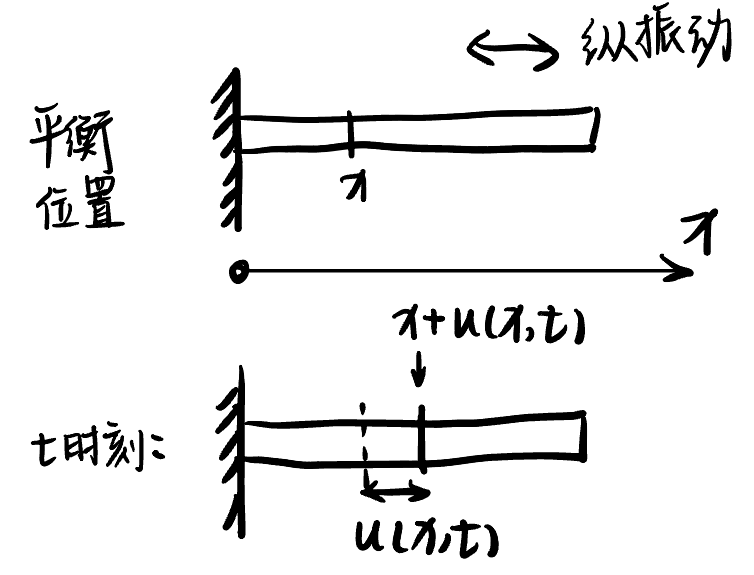
\includegraphics[width=0.3\textwidth]{figures/Stick.png} %插入图片,[]中设置图片大小,{}中是图片文件名
    \label{stick} %用于文内引用的标签
\end{figure}%结束环境
单位面积上的拉力$\boxed{p=E\dfrac{\partial{u}}{\partial{x}}}$,以向右为正($E$:杨氏模量)

合力
$$
\begin{aligned}
    &F_{\mbox{合}}=p(x+\Delta x,t)S-p(x,t)S\\
    =&S\left(E|_{x+\Delta x}\frac{\partial{u}}{\partial{x}}\bigg|_{x+\Delta x}-E|_x\frac{\partial{u}}{\partial{x}}\bigg|_x\right)\\
    =&S\frac{\partial}{\partial x}\left(E\frac{\partial u}{\partial x}\right)
    \xlongequal{E=\mathrm{const}} ES \frac{\partial^2{{u}}}{\partial{x}^2}\Delta x
\end{aligned}$$

根据牛二定律:
$$F_{\mbox{合}}=\rho S\Delta x \frac{\partial^2{\bar{u}}}{\partial{t}^2}$$

得到波动方程:
$$E \frac{\partial^2{u}}{\partial{x}^2}=\rho\frac{\partial^2{u}}{\partial{t}^2}$$

作变量代换$a=\sqrt{\dfrac{E}{\rho}}$

$$\boxed{\frac{\partial^2{u}}{\partial{t}^2}=a^2\frac{\partial^2{u}}{\partial{x}^2}}$$



